% Technical Report for OSINT Tool All-in-One
% Author: Vu Van Nam, Nguyen Cong Son
% Class: IT3910E - 750639
% Instructor: Hoang Viet Dung

\documentclass[13pt,a4paper]{report}
\usepackage[utf8]{inputenc}
\usepackage{graphicx}
\usepackage{hyperref}
\usepackage{geometry}
\geometry{left=3cm,right=2.5cm,top=2.5cm,bottom=2.5cm}
\usepackage{setspace}
\usepackage{titlesec}
\usepackage{fancyhdr}
\usepackage{caption}
\usepackage{enumitem}
\usepackage{listings}
\usepackage{color}
\usepackage{booktabs}
\usepackage{tikz}
\usetikzlibrary{positioning, shapes, arrows}

\titleformat{\chapter}[display]{\bfseries\Huge}{\chaptername\ \thechapter}{20pt}{\Huge}
\renewcommand{\baselinestretch}{1.3}

%--------------------
% Cover Page
%--------------------
\begin{document}

\begin{titlepage}
    \centering
    % Logo HUST
    
\includegraphics[width=0.25\textwidth]{hust_logo.jpg} \\[1.5cm]
    {\Large \textbf{HANOI UNIVERSITY OF SCIENCE AND TECHNOLOGY}} \\[0.5cm]
    {\large \textbf{SCHOOL OF INFORMATION AND COMMUNICATION TECHNOLOGY}} \\[1.5cm]
    {\Huge \textbf{Technical Report}} \\[0.5cm]
    {\LARGE \textbf{OSINT Tool All-in-One: Social Network Reconnaissance Program Development}} \\[1.5cm]
    \begin{flushleft}
        {\large \textbf{Course:} IT3910E -- Class code: 750639} \\[0.75cm]
        {\large \textbf{Instructor:} Hoang Viet Dung} \\[0.75cm]
        {\large \textbf{Group Members:}} \\ [0.5cm]
        {\large \ \ \ Vu Van Nam -- 20235610 -- Nam.VV235610@sis.hust.edu.vn} \\[0.5cm]
        {\large \ \ \ Nguyen Cong Son -- 20235619 -- Son.NC235619@sis.hust.edu.vn} \\[0.5cm]
    \end{flushleft}
    \vfill
    Hanoi, 2025
\end{titlepage}

%--------------------
% Abstract
%--------------------
\begin{abstract}
This report presents the design and implementation of the "OSINT Tool All-in-One" project, which aims to automate the process of collecting, analyzing, and visualizing social network data for reconnaissance purposes. The tool leverages both API-based and browser-based crawling techniques to extract user information, friend networks, and statistical insights from Facebook. The system is built with a modular architecture, supports data visualization, and is designed to be extensible for future AI-powered analysis. The report details the system architecture, main features, technologies used, challenges encountered, and experimental results.
\end{abstract}

\tableofcontents
\newpage

%--------------------
% Introduction
%--------------------
\chapter{Introduction}
\section{Background}
Open Source Intelligence (OSINT) is the process of collecting and analyzing publicly available information for intelligence purposes. With the rapid growth of social networks, OSINT tools have become essential for security, research, and investigative tasks. Social networks like Facebook, Twitter, and LinkedIn contain vast amounts of user-generated data, which can be leveraged for various purposes such as threat detection, market research, and social analysis.

\section{Motivation}
The increasing complexity and volume of social network data present both opportunities and challenges. Manual data collection is time-consuming and error-prone. Therefore, there is a strong need for automated tools that can efficiently gather, process, and visualize social network information. This project aims to address these needs by developing an all-in-one OSINT tool focused on Facebook.

\section{Related Work}
Several OSINT tools exist, such as Maltego, SpiderFoot, and Recon-ng. While these tools offer powerful features, they often require complex setup or are limited in their ability to extract deep social network data due to API restrictions. Our tool differentiates itself by combining both API-based and browser-based crawling, allowing for more comprehensive data extraction.

\section{Report Structure}
This report is organized as follows:
\begin{itemize}
    \item Chapter 1: Introduction
    \item Chapter 2: Objectives and Scope
    \item Chapter 3: System Analysis
    \item Chapter 4: System Design and Implementation
    \item Chapter 5: Main Features
    \item Chapter 6: Implementation Process
    \item Chapter 7: Installation and Usage Guide
    \item Chapter 8: Results and Evaluation
    \item Chapter 9: Discussion and Recommendations
    \item Chapter 10: References
\end{itemize}

%--------------------
% Objectives and Scope
%--------------------
\chapter{Objectives and Scope}
\section{Project Objectives}
The main objectives of this project are:
\begin{itemize}
    \item To develop a tool that can automatically collect friend lists and personal information from Facebook accounts.
    \item To provide both API-based and browser-based crawling methods for data extraction.
    \item To visualize social network structures and statistical distributions (e.g., by province).
    \item To extract location-based information including check-in data and movement patterns from user profiles.
    \item To generate comprehensive movement timeline statistics and travel behavior analysis.
    \item To support extensibility for future AI-based analysis and deeper data mining.
\end{itemize}

\section{Scope of Work}
The scope of the project is limited to publicly accessible Facebook data and does not involve any unauthorized access or data breaches. The tool is designed for educational and research purposes, adhering to ethical guidelines and respecting user privacy.

\section{Expected Outcomes}
\begin{itemize}
    \item A fully functional OSINT tool capable of extracting and visualizing Facebook social network data.
    \item Documentation and user guide for easy deployment and usage.
    \item Experimental results demonstrating the effectiveness of the tool.
\end{itemize}

%--------------------
% System Analysis
%--------------------
\chapter{System Analysis}
\section{Problem Definition}
In the digital age, social networking platforms have become repositories of vast amounts of publicly available information about individuals and their relationships. Facebook, with over 2.9 billion active users, contains rich datasets including user profiles, friendship networks, geographic locations, and movement patterns. However, extracting and analyzing this information for legitimate purposes such as cybersecurity investigations, social research, or business intelligence remains a significant challenge.

Currently, most data collection processes are performed manually, which is extremely time-consuming and error-prone. Researchers and security professionals often spend countless hours manually browsing profiles, collecting friend lists, and analyzing relationships without systematic tools. Existing OSINT tools, while powerful, are often limited by API restrictions, require complex technical setup, or lack comprehensive features for social network analysis.

The necessity of developing an automated OSINT tool becomes evident when considering the scale and complexity of modern social networks. Manual analysis of even a modest network of 100-200 users and their connections can take weeks to complete. Furthermore, identifying patterns such as geographic clustering, movement timelines, or relationship hierarchies is nearly impossible without proper visualization and statistical analysis tools.

The real-world significance of this project extends across multiple domains. For cybersecurity professionals, the tool enables rapid threat assessment and social engineering vulnerability analysis. Academic researchers can leverage it for studying social dynamics, migration patterns, and community structures. Law enforcement agencies can utilize it for digital forensics and investigation support, while businesses can apply it for market research and competitor analysis.

By automating the data collection and analysis process, this tool addresses the critical gap between the abundance of social media data and the practical ability to extract meaningful insights from it. The system's capability to visualize complex social networks and generate statistical reports transforms raw data into actionable intelligence, significantly enhancing the efficiency and effectiveness of OSINT operations.

\section{Target Users and Usage Scenarios}
\subsection{Target User Groups}
The OSINT Tool All-in-One is designed for diverse user groups with varying technical backgrounds and requirements:

\textbf{Cybersecurity Professionals:} Security analysts, penetration testers, and cybersecurity consultants who need to assess social engineering vulnerabilities, investigate suspicious accounts, or analyze potential threat actors. These users typically have moderate technical skills and prefer both command-line efficiency and web-based visualization.

\textbf{Academic Researchers:} Social scientists, digital humanities scholars, and data analysts studying social networks, migration patterns, or online behavior. They require comprehensive data collection capabilities and statistical analysis tools but may prefer user-friendly web interfaces over command-line operations.

\textbf{Digital Forensics Investigators:} Law enforcement personnel, private investigators, and forensics specialists who need to gather evidence, trace connections between suspects, or reconstruct timelines of activities. They often work under time constraints and need reliable, documented processes.

\textbf{Business Intelligence Analysts:} Marketing professionals, competitive analysts, and market researchers who want to understand customer behavior, analyze competitor networks, or identify influencers in specific geographic regions.

\textbf{Students and Educators:} Computer science students, cybersecurity trainees, and instructors teaching OSINT techniques who need hands-on experience with real-world data collection and analysis tools.

\subsection{Typical Usage Scenarios}

\textbf{Scenario 1: Corporate Security Assessment}
A cybersecurity consultant needs to evaluate social engineering risks for a client company. Using the tool, they collect employee social networks, analyze geographic distribution, and identify potential attack vectors through friendship connections. The process involves using clone Facebook accounts, setting crawling parameters (2-3 layers, 50-100 friends per node), and generating visual reports for management presentation.

\textbf{Scenario 2: Academic Social Network Research}
A sociology researcher studying urban migration patterns uses the tool to collect location data and movement timelines from public Facebook profiles. They utilize the web interface to configure data collection, export results to JSON format for statistical analysis, and generate HTML visualizations to illustrate migration flows between cities.

\textbf{Scenario 3: Digital Investigation}
A digital forensics investigator needs to trace connections between suspected individuals in a fraud case. They use the command-line interface for systematic data collection, analyze friendship networks to identify key intermediaries, and document movement patterns using timeline statistics. The investigation requires processing hundreds of profiles while maintaining evidence integrity.

\textbf{Scenario 4: Market Research Campaign}
A marketing team wants to understand social connections within their target demographic in specific provinces. They use the web interface to collect and visualize geographic distribution, identify local influencers, and analyze social clustering patterns to optimize their advertising strategy.

\textbf{Scenario 5: Educational Training}
An instructor teaching OSINT techniques uses the tool to demonstrate real-world data collection methods. Students learn to operate both command-line and web interfaces, understand the ethical implications of data gathering, and practice generating comprehensive reports from social media intelligence.

\section{Use-Case Analysis}
The use-case diagram illustrates the primary functional requirements of the OSINT Tool system through the lens of user-system interactions. The diagram identifies five distinct actor types and seven core use cases that represent the system's fundamental capabilities for social network intelligence gathering and analysis.

\begin{figure}[h!]
    \centering
    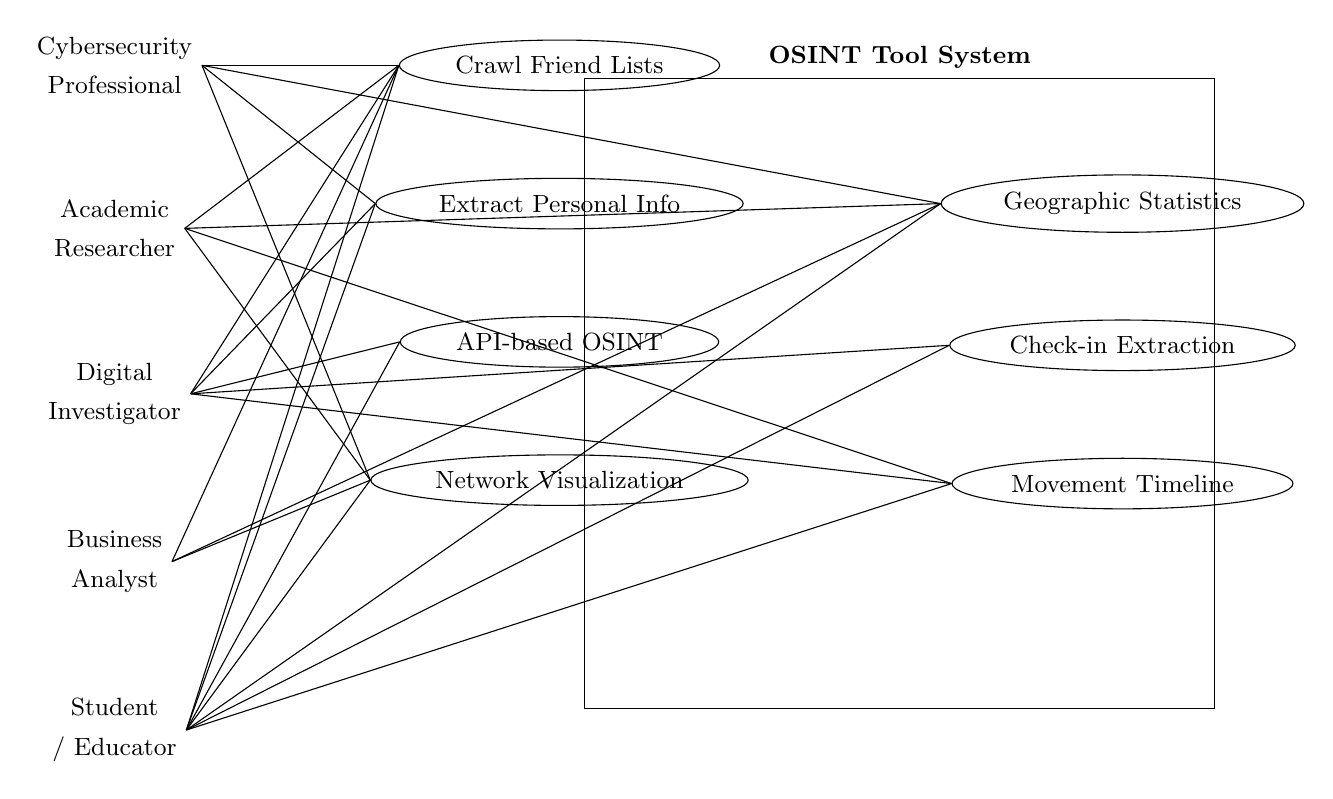
\begin{tikzpicture}[node distance=1.1cm and 1.2cm, every node/.style={font=\small}]
        % Actors
        \node (A1) [align=center] {Cybersecurity\\Professional};
        \node (A2) [align=center, below=of A1] {Academic\\Researcher};
        \node (A3) [align=center, below=of A2] {Digital\\Investigator};
        \node (A4) [align=center, below=of A3] {Business\\Analyst};
        \node (A5) [align=center, below=of A4] {Student\\/ Educator};

        % System boundary
        \node[draw, rectangle, minimum width=8cm, minimum height=8cm, right=5cm of A3, label=above:{\textbf{OSINT Tool System}}] (system) {};

        % Use cases inside system
        \node[draw, ellipse, right=2.5cm of A1.east] (UC1) {Crawl Friend Lists};
        \node[draw, ellipse, below=of UC1] (UC2) {Extract Personal Info};
        \node[draw, ellipse, below=of UC2] (UC3) {API-based OSINT};
        \node[draw, ellipse, below=of UC3] (UC4) {Network Visualization};
        \node[draw, ellipse, right=2.5cm of UC2] (UC5) {Geographic Statistics};
        \node[draw, ellipse, below=of UC5] (UC6) {Check-in Extraction};
        \node[draw, ellipse, below=of UC6] (UC7) {Movement Timeline};

        % Relationships for A1
        \draw (A1.east) -- (UC1.west);
        \draw (A1.east) -- (UC2.west);
        \draw (A1.east) -- (UC4.west);
        \draw (A1.east) -- (UC5.west);

        % Relationships for A2
        \draw (A2.east) -- (UC1.west);
        \draw (A2.east) -- (UC4.west);
        \draw (A2.east) -- (UC5.west);
        \draw (A2.east) -- (UC7.west);

        % Relationships for A3
        \draw (A3.east) -- (UC1.west);
        \draw (A3.east) -- (UC2.west);
        \draw (A3.east) -- (UC3.west);
        \draw (A3.east) -- (UC6.west);
        \draw (A3.east) -- (UC7.west);

        % Relationships for A4
        \draw (A4.east) -- (UC1.west);
        \draw (A4.east) -- (UC4.west);
        \draw (A4.east) -- (UC5.west);

        % Relationships for A5
        \draw (A5.east) -- (UC1.west);
        \draw (A5.east) -- (UC2.west);
        \draw (A5.east) -- (UC3.west);
        \draw (A5.east) -- (UC4.west);
        \draw (A5.east) -- (UC5.west);
        \draw (A5.east) -- (UC6.west);
        \draw (A5.east) -- (UC7.west);
    \end{tikzpicture}
    \caption{Use-case diagram of the OSINT Tool system.}
\end{figure}

\subsection{Actor Definitions}
The system serves five primary actor categories, each with distinct objectives and interaction patterns:

\textbf{Cybersecurity Professional:} Focuses on threat assessment and vulnerability analysis. Primary interactions involve friend network crawling to identify attack vectors, personal information extraction for social engineering risk evaluation, and network visualization to understand organizational exposure.

\textbf{Academic Researcher:} Concentrates on social science studies and demographic analysis. Key interactions include geographic statistics generation for migration studies, movement timeline analysis for behavioral research, and comprehensive data export for statistical modeling.

\textbf{Digital Investigator:} Requires comprehensive intelligence gathering capabilities. Utilizes all system functions extensively, with particular emphasis on API-based OSINT for evidence collection, check-in data extraction for timeline reconstruction, and systematic data documentation for legal proceedings.

\textbf{Business Analyst:} Emphasizes market intelligence and competitive analysis. Primary interactions focus on network visualization for influence mapping, geographic statistics for market segmentation, and relationship analysis for customer behavior understanding.

\textbf{Student/Educator:} Engages with the system for educational purposes. Interactions span all use cases to provide comprehensive learning experiences in OSINT techniques, ethical data collection practices, and intelligence analysis methodologies.

\subsection{Use Case Descriptions}
\textbf{UC1 - Crawl Friend Lists:} The foundational use case enabling systematic collection of social network connections. Users specify target profiles, crawling depth (1-3 layers), and friend limits per node. The system employs Selenium automation to navigate Facebook's interface and extract friendship data while respecting rate limits and detection avoidance.

\textbf{UC2 - Extract Personal Information:} Builds upon crawled networks to gather detailed profile data. Users select target individuals from collected friend lists, triggering automated extraction of public information including demographics, education, employment, and location history.

\textbf{UC3 - Perform API-based OSINT:} Provides access to Facebook's official APIs for post collection, comment analysis, and engagement metrics. Users select from available API scripts, configure parameters, and receive structured JSON outputs suitable for further analysis.

\textbf{UC4 - Generate Network Visualization:} Transforms collected data into interactive visual representations. The system produces force-directed graphs with customizable layouts, node filtering capabilities, and export options for presentations or further analysis tools.

\textbf{UC5 - Analyze Geographic Statistics:} Processes location data to generate statistical insights about geographic distribution patterns. Outputs include province-based demographics, migration flow analysis, and geographic clustering identification.

\textbf{UC6 - Extract Check-in Data:} Specialized function for location intelligence gathering. Parses Facebook check-in information, geo-tags, and location metadata to build comprehensive movement profiles for individuals within the network.

\textbf{UC7 - Generate Movement Timeline:} Advanced analytical capability combining check-in data with temporal analysis. Creates chronological visualizations of movement patterns, identifies frequently visited locations, and detects behavioral anomalies or travel patterns.

\subsection{Interaction Workflows}
The system supports both sequential and parallel use case execution. A typical analytical workflow begins with UC1 (friend list crawling) as the data foundation, followed by UC2 (personal information extraction) for enrichment. Subsequently, users can execute UC4, UC5, UC6, and UC7 in parallel or sequentially based on analytical objectives.

Cross-cutting interactions occur through shared data repositories, enabling seamless transitions between use cases without data re-collection. The system maintains data lineage and provenance tracking, ensuring audit trails for investigative and research applications. Each use case generates standardized outputs (JSON, HTML, CSV) facilitating integration with external analytical tools and workflows.

%--------------------
% System Design and Implementation
%--------------------
\chapter{System Design and Implementation}

\section{Technology Selection and Rationale}
The system leverages a modern, open-source technology stack chosen for its robustness, community support, and suitability for large-scale data processing and interactive visualization:
\begin{itemize}
    \item \textbf{Python 3.10}: Primary backend language due to its rich ecosystem for web scraping, data analysis, and rapid prototyping.
    \item \textbf{Selenium}: Enables browser automation to bypass API limitations and mimic human interaction when collecting friend lists, check-ins, and other semi-private data.
    \item \textbf{FastAPI}: Lightweight, high-performance Python web framework used to expose RESTful endpoints for the frontend and external integrations.
    \item \textbf{NetworkX \,\&\, Matplotlib}: Provide graph data structures and visual analytics for network topology and statistical plots.
    \item \textbf{React + Vite + TailwindCSS}: Implement an SPA dashboard for interactive exploration of collected data. Vite offers fast HMR while Tailwind ensures consistent styling.
    \item \textbf{D3.js}: Powers advanced, dynamic visualizations (force-directed graphs, choropleth maps, timelines).
    \item \textbf{Docker}: Optional containerization for reproducible deployment across environments.
\end{itemize}
These choices minimize licensing costs, accelerate development, and ensure the tool can be easily extended or integrated with future AI modules.

\section{System Implementation and Configuration}
\begin{figure}[h!]
    \centering
    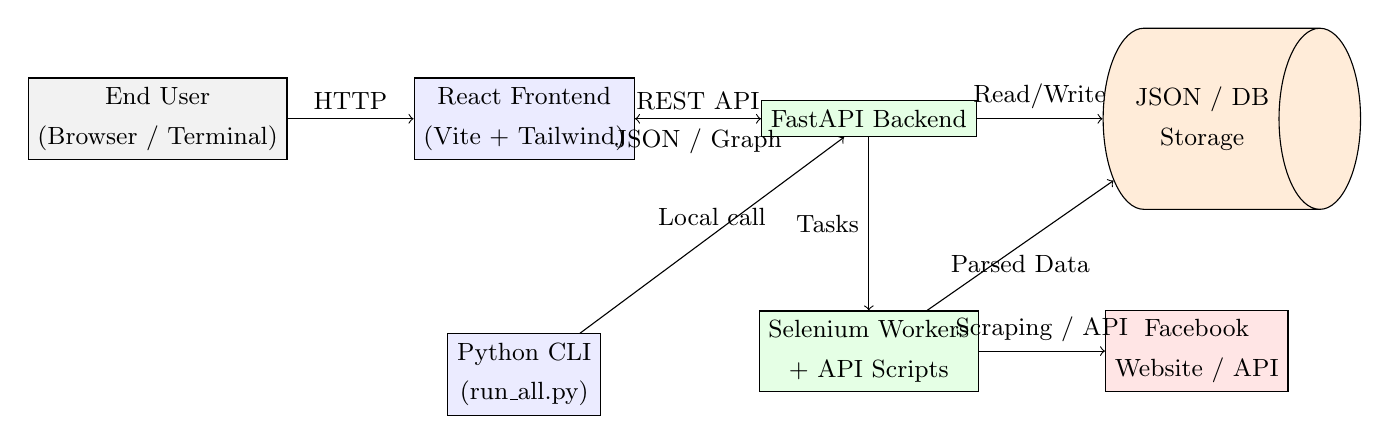
\begin{tikzpicture}[node distance=2.2cm and 1.6cm, every node/.style={font=\small}]
        % Layers
        % User layer
        \node (User) [draw, rectangle, align=center, fill=gray!10] {End User\\(Browser / Terminal)};

        % Frontend & CLI
        \node (Web) [draw, rectangle, right=of User, align=center, fill=blue!8] {React Frontend\\(Vite + Tailwind)};
        \node (CLI) [draw, rectangle, below=of Web, align=center, fill=blue!8] {Python CLI\\(run\_all.py)};

        % Backend layer
        \node (API) [draw, rectangle, right=of Web, align=center, fill=green!10] {FastAPI Backend};
        \node (Worker) [draw, rectangle, below=of API, align=center, fill=green!10] {Selenium Workers\\+ API Scripts};

        % Storage layer
        \node (Storage) [draw, cylinder, right=of API, align=center, fill=orange!15, minimum height=1.4cm, minimum width=2.3cm] {JSON / DB\\Storage};

        % External
        \node (Facebook) [draw, rectangle, right=of Worker, align=center, fill=red!10] {Facebook\\Website / API};

        % Arrows
        \draw[->] (User) -- node[above] {HTTP} (Web);
        \draw[->] (Web) -- node[above] {REST API} (API);
        \draw[->] (CLI) -- node[above] {Local call} (API);
        \draw[->] (API) -- node[left] {Tasks} (Worker);
        \draw[->] (Worker) -- node[above] {Scraping / API} (Facebook);
        \draw[->] (Worker) -- node[below] {Parsed Data} (Storage);
        \draw[->] (API) -- node[above] {Read/Write} (Storage);
        \draw[<-] (Web) -- node[below] {JSON / Graph} (API);
    \end{tikzpicture}
    \caption{System Architecture Diagram of OSINT Tool All-in-One.}
    \label{fig:architecture}
\end{figure}

\section{Feature Survey and User Interactions}
Table~\ref{tab:feature-survey} summarises the key features and how each user group typically interacts with them.

\begin{table}[h!]
    \centering
    \caption{Feature survey and corresponding user interactions}
    \label{tab:feature-survey}
    \begin{tabular}{@{}llp{7.5cm}@{}}
        \toprule
        \textbf{Feature} & \textbf{Main Interface} & \textbf{Typical Interaction} \\ \midrule
        Friend list crawling & CLI / Web & User specifies root UID, depth, and friend limit; system launches Selenium workers and streams progress. \\
        Personal info extraction & CLI / Web & After crawling, user triggers profile scraping; results exported as JSON. \\
        API-based OSINT & CLI / Web & User selects API script (e.g., posts, comments); output saved to structured files. \\
        Network visualization & CLI / Web & Interactive force-directed graph with node filtering, search, and legend. \\
        Geographic statistics & CLI / Web & Choropleth map and pie charts showing province distribution. \\
        Check-in extraction & CLI / Web & Locations parsed, stored with timestamps for timeline analysis. \\
        Movement timeline & CLI / Web & Scrollable timeline chart displaying movement events per user. \\
        \bottomrule
    \end{tabular}
\end{table}

%--------------------
% Main Features
%--------------------
\chapter{Main Features}
\section{Friend List Crawling}
The tool allows users to input a Facebook UID or username and specify the number of layers and friends per node to crawl. The crawling process is automated using Selenium, which simulates browser actions to extract friend lists even when API access is restricted.

\begin{lstlisting}[language=Python, caption=Example: Initiating Friend List Crawling]
python run_all.py
# Follow the menu to select friend list crawling
\end{lstlisting}

\section{Personal Information Extraction}
After collecting friend lists, the tool can extract detailed personal information for each user in the network. This includes public profile data such as name, location, education, and work history.

\section{API-based OSINT}
The tool includes several API scripts for extracting posts, comments, and profile details. Users can select which API script to run, and the results are saved in structured JSON files for further analysis.

\section{Network Visualization}
The tool generates an interactive HTML network graph, allowing users to explore the structure of the social network visually. Nodes represent users, and edges represent friendship connections. The root user is highlighted for easy identification.

\section{Geographic Statistics}
The tool provides province-based statistics and other analytical insights from the data. For example, users can view the distribution of friends by province, helping to identify geographic patterns in the network.

\section{Check-in Data Extraction}
The tool extracts location check-in data from user profiles, storing the information with timestamps for timeline analysis. This feature allows researchers to track movement patterns and geographic presence of subjects over time.

\section{Movement Timeline}
The tool provides a scrollable timeline chart that displays movement events for each user. This visualization helps analysts track subjects' movements over time, identify patterns, and understand geographic behaviors through an intuitive chronological interface.

\section{Terminal Interface}
The terminal interface provides a simple command-line menu for users to select the desired function. This interface is ideal for technical users and automation tasks. Below is a screenshot of the main terminal menu:
\begin{figure}[h!]
    \centering
    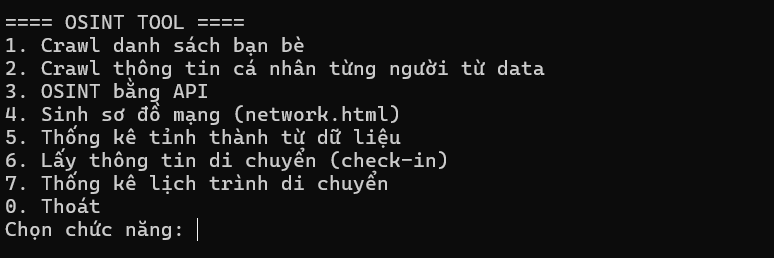
\includegraphics[width=0.7\textwidth]{4.png}
    \caption{Terminal interface of OSINT Tool All-in-One.}
\end{figure}

\section{Web Interface}
The web interface provides a modern, user-friendly dashboard for data visualization and analysis. Users can access network graphs, geographic statistics, and movement timelines through an intuitive browser-based UI. The responsive design works across desktop and mobile devices, making it accessible for field operations.
\begin{figure}[h!]
    \centering
    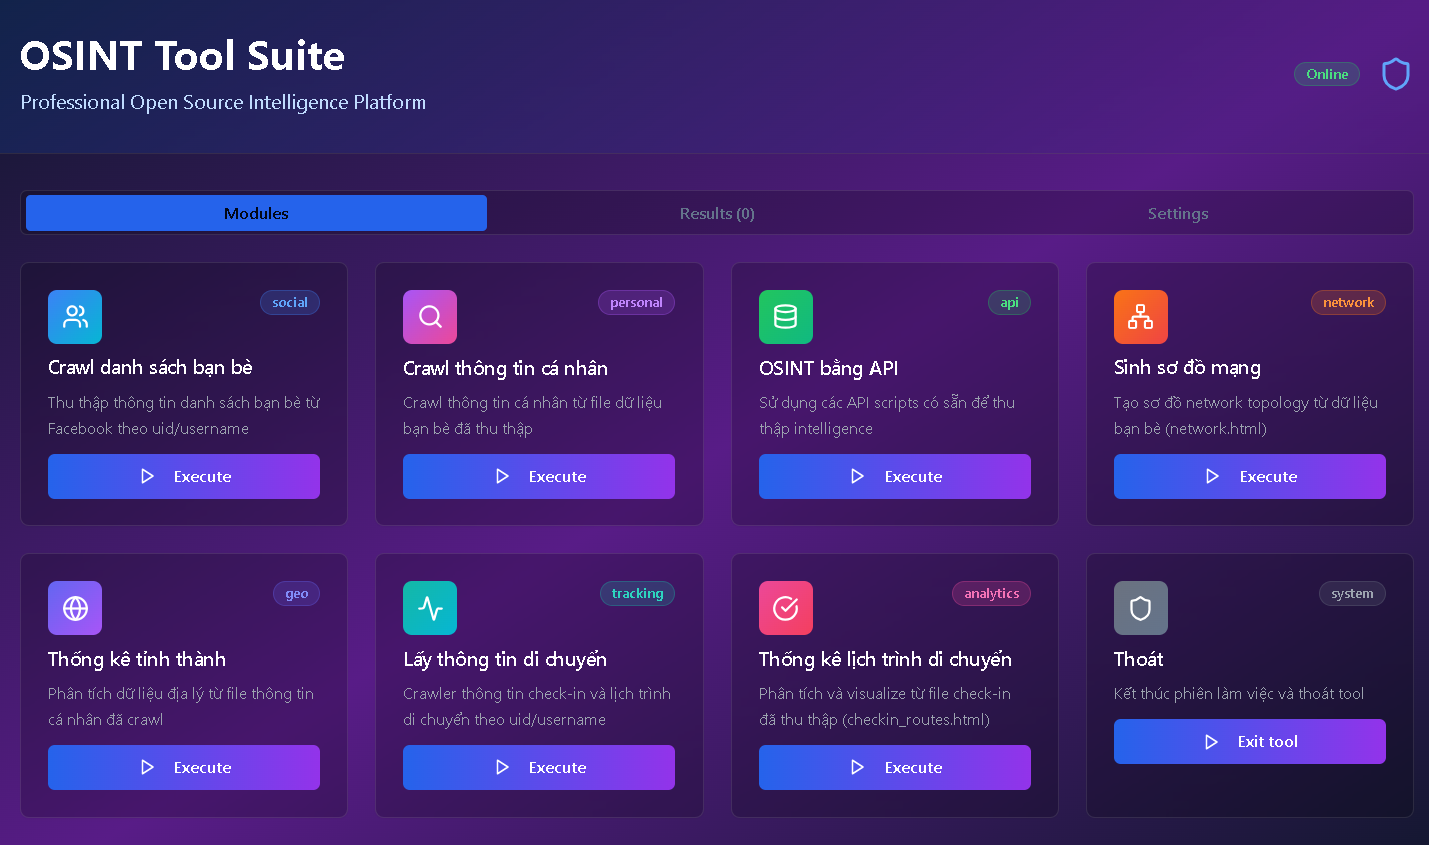
\includegraphics[width=0.95\textwidth]{web_dashboard.png}
    \caption{Web interface dashboard of OSINT Tool All-in-One showing the main features.}
\end{figure}

%--------------------
% Implementation Process
%--------------------
\chapter{Implementation Process}
\section{Project Timeline and Work Distribution}
% TODO: Detail the phases of the project, timeline (Gantt chart), and contribution of each member.

The project was executed over a period of approximately 7 weeks, from April 20th to June 9th, 2024. The development process was divided into three main phases, with both team members contributing equally (50-50) to the overall project outcomes.

\subsection{Phase 1: Research and Analysis (April 20 - May 4, 2024)}
\textbf{Duration:} 2 weeks \\
\textbf{Objective:} Investigate available Facebook APIs and assess their capabilities for OSINT purposes.

During this initial phase, both team members conducted extensive research into Facebook's API ecosystem. The investigation revealed significant limitations in the official APIs, including:
\begin{itemize}
    \item Restricted access to friend list data
    \item Limited personal information retrieval capabilities  
    \item Rate limiting and authentication barriers
    \item Insufficient data granularity for comprehensive OSINT analysis
\end{itemize}

While the APIs offered speed advantages, their restricted nature made them unsuitable for the project's comprehensive intelligence gathering requirements.

\subsection{Phase 2: Development and Implementation (May 5 - May 25, 2024)}
\textbf{Duration:} 3 weeks \\
\textbf{Objective:} Develop alternative crawling methods and implement core features.

Following the API research conclusions, the team pivoted to browser-based crawling solutions. \textbf{Vu Van Nam} spearheaded the research into alternative crawling methodologies, drawing inspiration from the MetaSpy framework to develop a Selenium-based approach capable of bypassing API restrictions.

Simultaneously, \textbf{Nguyen Cong Son} continued exploring API-based solutions to identify any remaining viable endpoints. Once the crawling foundation was established, both members collaborated on implementing the core features:

\begin{itemize}
    \item Friend list crawling algorithms
    \item Personal information extraction modules
    \item Geographic statistics generation
    \item Check-in data extraction and movement tracking
    \item Network visualization components
\end{itemize}

\textbf{Division of Expertise:}
\begin{itemize}
    \item \textbf{Vu Van Nam:} Lead developer for crawling methodology research and implementation
    \item \textbf{Nguyen Cong Son:} Primary developer for API-based OSINT features and integration
\end{itemize}

\subsection{Phase 3: Refinement and Finalization (May 26 - June 9, 2024)}
\textbf{Duration:} 2 weeks \\
\textbf{Objective:} System optimization, quality assurance, and documentation.

The final phase focused on system refinement and project deliverables:

\textbf{Joint Activities:}
\begin{itemize}
    \item Collaborative debugging and error resolution
    \item Code optimization and performance tuning
    \item Integration testing and system validation
\end{itemize}

\textbf{Individual Responsibilities:}
\begin{itemize}
    \item \textbf{Vu Van Nam:} SonarQube configuration, CI/CD pipeline setup, project documentation and report preparation
    \item \textbf{Nguyen Cong Son:} Web interface development, user experience optimization, and frontend integration
\end{itemize}

\subsection{Work Distribution Summary}
Both team members contributed equally to the project's success, with a 50-50 work distribution across all phases. The collaboration was characterized by complementary skill sets and shared responsibility for critical system components, ensuring robust development and comprehensive feature implementation.

\section{Continuous Integration / Continuous Deployment (CI/CD)}
% TODO: Describe the CI/CD pipeline configuration and tools used (e.g., GitHub Actions, Docker).
\begin{figure}[h!]
    \centering
    
\includegraphics[width=0.9\textwidth]{6.png}
    \caption{CI/CD pipeline execution summary.}
\end{figure}

\section{Static Code Analysis}
% TODO: Include SonarQube or similar analysis results.
\begin{figure}[h!]
    \centering
    
\includegraphics[width=0.8\textwidth]{7.png}
    \caption{SonarQube report highlighting code quality metrics.}
\end{figure}

%--------------------
% Installation and Usage Guide
%--------------------
\chapter{Installation and Usage Guide}
\section{Backend Setup}
\subsection{Python Environment}
\begin{enumerate}
    \item Install Python 3.8+ and required packages:
    \begin{verbatim}
    pip install -r requirements.txt
    \end{verbatim}
    \item Set up environment variables for Facebook account and API if needed.
    \item Run the main tool:
    \begin{verbatim}
    python run_all.py
    \end{verbatim}
    \item Follow the on-screen menu instructions.
\end{enumerate}

\subsection{Troubleshooting}
Common issues include missing dependencies, incorrect environment variables, or browser driver errors. Ensure all required packages are installed and the correct version of ChromeDriver is used.

\section{Frontend Setup}
\begin{enumerate}
    \item Install Node.js and npm.
    \item Navigate to the visualization directory:
    \begin{verbatim}
    cd "tsx hometown/map"
    npm install
    npm run build
    npx serve dist
    \end{verbatim}
    \item Open your browser and go to http://localhost:3000
\end{enumerate}

\subsection{Usage Tips}
- Always run the tool from the project root directory.
- Data files are saved with timestamps to avoid overwriting.
- If login issues occur, check cookies and try logging in manually via Chrome.

%--------------------
% Results and Evaluation
%--------------------
\chapter{Results and Evaluation}
\section{Test Scenarios}
Several test scenarios were conducted to evaluate the tool's performance and accuracy:
\begin{itemize}
    \item Crawling friend lists for accounts with varying numbers of friends.
    \item Extracting detailed profile information for selected users.
    \item Running API scripts to collect posts and comments.
    \item Visualizing large and small social networks.
\end{itemize}

\section{Results and Analysis}
The tool successfully collected and visualized social network data for multiple test accounts. The network graph visualization provided clear insights into the structure and key nodes within the network. Province-based statistics highlighted geographic trends among friends.

\begin{table}[h!]
    \centering
    \caption{Sample Data Collection Results}
    \begin{tabular}{@{}lccc@{}}
        \toprule
        Test Case & Number of Friends & Layers Crawled & Time Taken (s) \\
        \midrule
        Account A & 150 & 2 & 45 \\
        Account B & 300 & 2 & 90 \\
        Account C & 50 & 1 & 12 \\
        \bottomrule
    \end{tabular}
\end{table}

\section{Screenshots}
\begin{figure}[h!]
    \centering
    
\includegraphics[width=0.95\textwidth]{2.png}
    \caption{Network graph visualization for a test account.}
\end{figure}

\begin{figure}[h!]
    \centering
    
\includegraphics[width=0.7\textwidth]{3.png}
    \caption{Province statistics visualization for the same account.}
\end{figure}

\section{Discussion}
The results demonstrate the tool's ability to handle different data sizes and provide meaningful visualizations. However, performance decreases with larger networks due to browser automation overhead. Further optimization is needed for large-scale data collection.

%--------------------
% Discussion and Recommendations
%--------------------
\chapter{Discussion and Recommendations}
\section{Challenges}
\begin{itemize}
    \item \textbf{Performance:} The tool runs slowly when collecting large amounts of data due to Java limitations and browser automation overhead.
    \item \textbf{API Restrictions:} Some APIs no longer allow extensive data extraction, requiring a switch to Python and browser-based crawling.
    \item \textbf{Data Quality:} Inconsistent or missing data from user profiles can affect analysis accuracy.
    \item \textbf{Maintenance:} Facebook interface changes may require updates to selectors and crawling logic.
\end{itemize}

\section{Future Work}
\begin{itemize}
    \item Integrate AI-based crawling to automatically understand and identify locations, special relationships, and more complex patterns in social networks.
    \item Optimize performance for large-scale data collection.
    \item Extend support to other social networks (e.g., Twitter, LinkedIn).
    \item Develop a web-based dashboard for real-time monitoring and analysis.
\end{itemize}

%--------------------
% References
%--------------------
\chapter{References}
\begin{itemize}
    \item meta-spy: \url{https://github.com/MetaCubeX/meta-spy}
    \item Maltego: \url{https://www.maltego.com/}
    \item SpiderFoot: \url{https://www.spiderfoot.net/}
    \item Recon-ng: \url{https://github.com/lanmaster53/recon-ng}
    \item Selenium: \url{https://www.selenium.dev/}
    \item NetworkX: \url{https://networkx.org/}
    \item FastAPI: \url{https://fastapi.tiangolo.com/}
\end{itemize}

\end{document} 